\section{A thermophysical model for a binary system of asteroids}
\label{sec:4}

In this section, we present the implementation of the mutual heating. As Didymos is a binary system of asteroid, the current thermophysical model is not enough to fully describe the temperature at the surface of the asteroid. The Hera mission focuses on the secondary object in this binary system. Its surface temperature depends also on the primary object for two main reasons, firstly, the reflection of the Sun on the surface of the primary to the secondary, this phenomenon depends on the primary albedo and on its position with respect to the Sun and the secondary, and it is named the mutual direct heating, and secondly, the heat received from the primary itself, just as the Sun, considering it as a black body, it only depend on the distance and is called the mutual diffuse heating.

\subsection{Theory}

Didymos’ secondary is modeled in a simplified manner due to the many unknowns and assumptions adopted in this study. This section deals with neglected effects thought to alter surface temperatures in certain cases.

A complete thermophysical model including the direct and diffuse mutual heating is \citep{pelivan}:
\begin{equation}
    Q_\odot+W_p+Q_p+W_m+Q_m=\epsilon\sigma u^4-k\frac{\partial{u}}{\partial{x}}\Big|_{x=0}
    \label{eq:4.1}
\end{equation}
where $W_p$ stands for the mutual heating from diffuse solar radiation from the primary, $Q_p$ corresponds to the direct thermal heating from the primary considered as a black body, $W_m$ is the diffuse thermal self heating, $Q_m$ is the direct thermal self heating and du/dx is the vertical temperature gradient with x positive upward.

For the current simplified model, the mutual heating from Didymain to Didymoon will be small due to the comparatively large distance of 1.18 km \citep{model} between the two bodies and enter through terms $W_p$ and $Q_p$. As defined in the reference model, the low albedo allows us to apply the single-scattering mode for which the diffuse thermal self heating flux $W_m$ can be neglected. Furthermore, considering the current shape of Didymoon, which is a simple ellipsoid, it is not necessary to include the term $Q_m$ neither. However, these two flux will be discussed in the next part.

Discretizing the two bodies into facets $i$ for the secondary and $j$ for the primary, the mutual heating from diffuse solar radiation from the primary can be compute using:
\begin{equation}
    W_p=\sum_{i\neq j}^N V_{ij}\frac{S_{\odot}A\cos\varsigma_j}{r_H^2}
    \label{eq:4.2}
\end{equation}
Where $N$ is the total number of facets and $V_{ij}$ is the view factor expressed as:
\begin{equation}
    V_{ij}=\frac{a_i\cos\theta_i\cos\theta_j}{\pi r^2}
    \label{eq:4.3}
\end{equation}
where $a_i$ is the surface area of the seconday, $r$ is the distance between facets $i$ and $j$ and angles $\theta$ are the angles between the facet outward normal and the line between facet centers from primary and seconday. An angle of $\theta\geq90$ degrees represents two facets not facing each other. The following schemes explain the situation:
\begin{figure*}[t]
    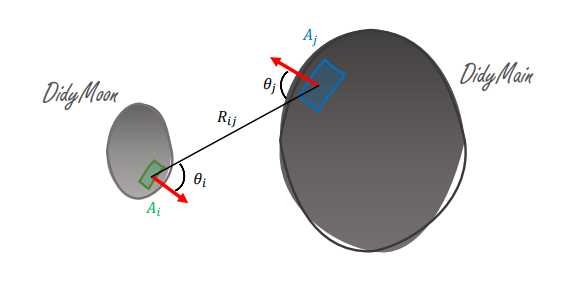
\includegraphics[width=0.6\linewidth]{rsc/viewfac1.png} 
    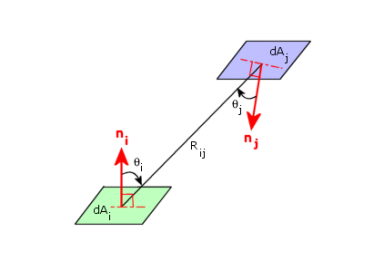
\includegraphics[width=0.6\linewidth]{rsc/viewfac2.png}
    \captionof{figure}{(1) View factor on Didymos system and (2) View factor schematic interpretation}
    \label{fig:4.1}
\end{figure*}

Due to low aldbedo (both albedo of the primary and secondary are assumed identical) the direct thermal heating $Q_p$ is the largest flux from the primary:
\begin{equation}
    Q_p=\sum_{i\neq j}^N V_{ij}\epsilon\sigma u^4_{j}
    \label{eq:4.4}
\end{equation}
where $u_{j}$ is the surface temperature of facet $j$. For computing time purposes, temperatures of the primary are not computed. All facets temperatures $u_{j}$ are set to the highest midday temperature of the moon. 

\subsection{Integration}
The \autoref{eq:4.1} can now be implemented to the current thermophysical model in \autoref{eq:2.1} to include the mutual heating from the primary body of the binary system of asteroid Didymos. Surface temperatures have been computed to each single node from the ESA shape models of the Didymos system asteroids.
\begin{center}
    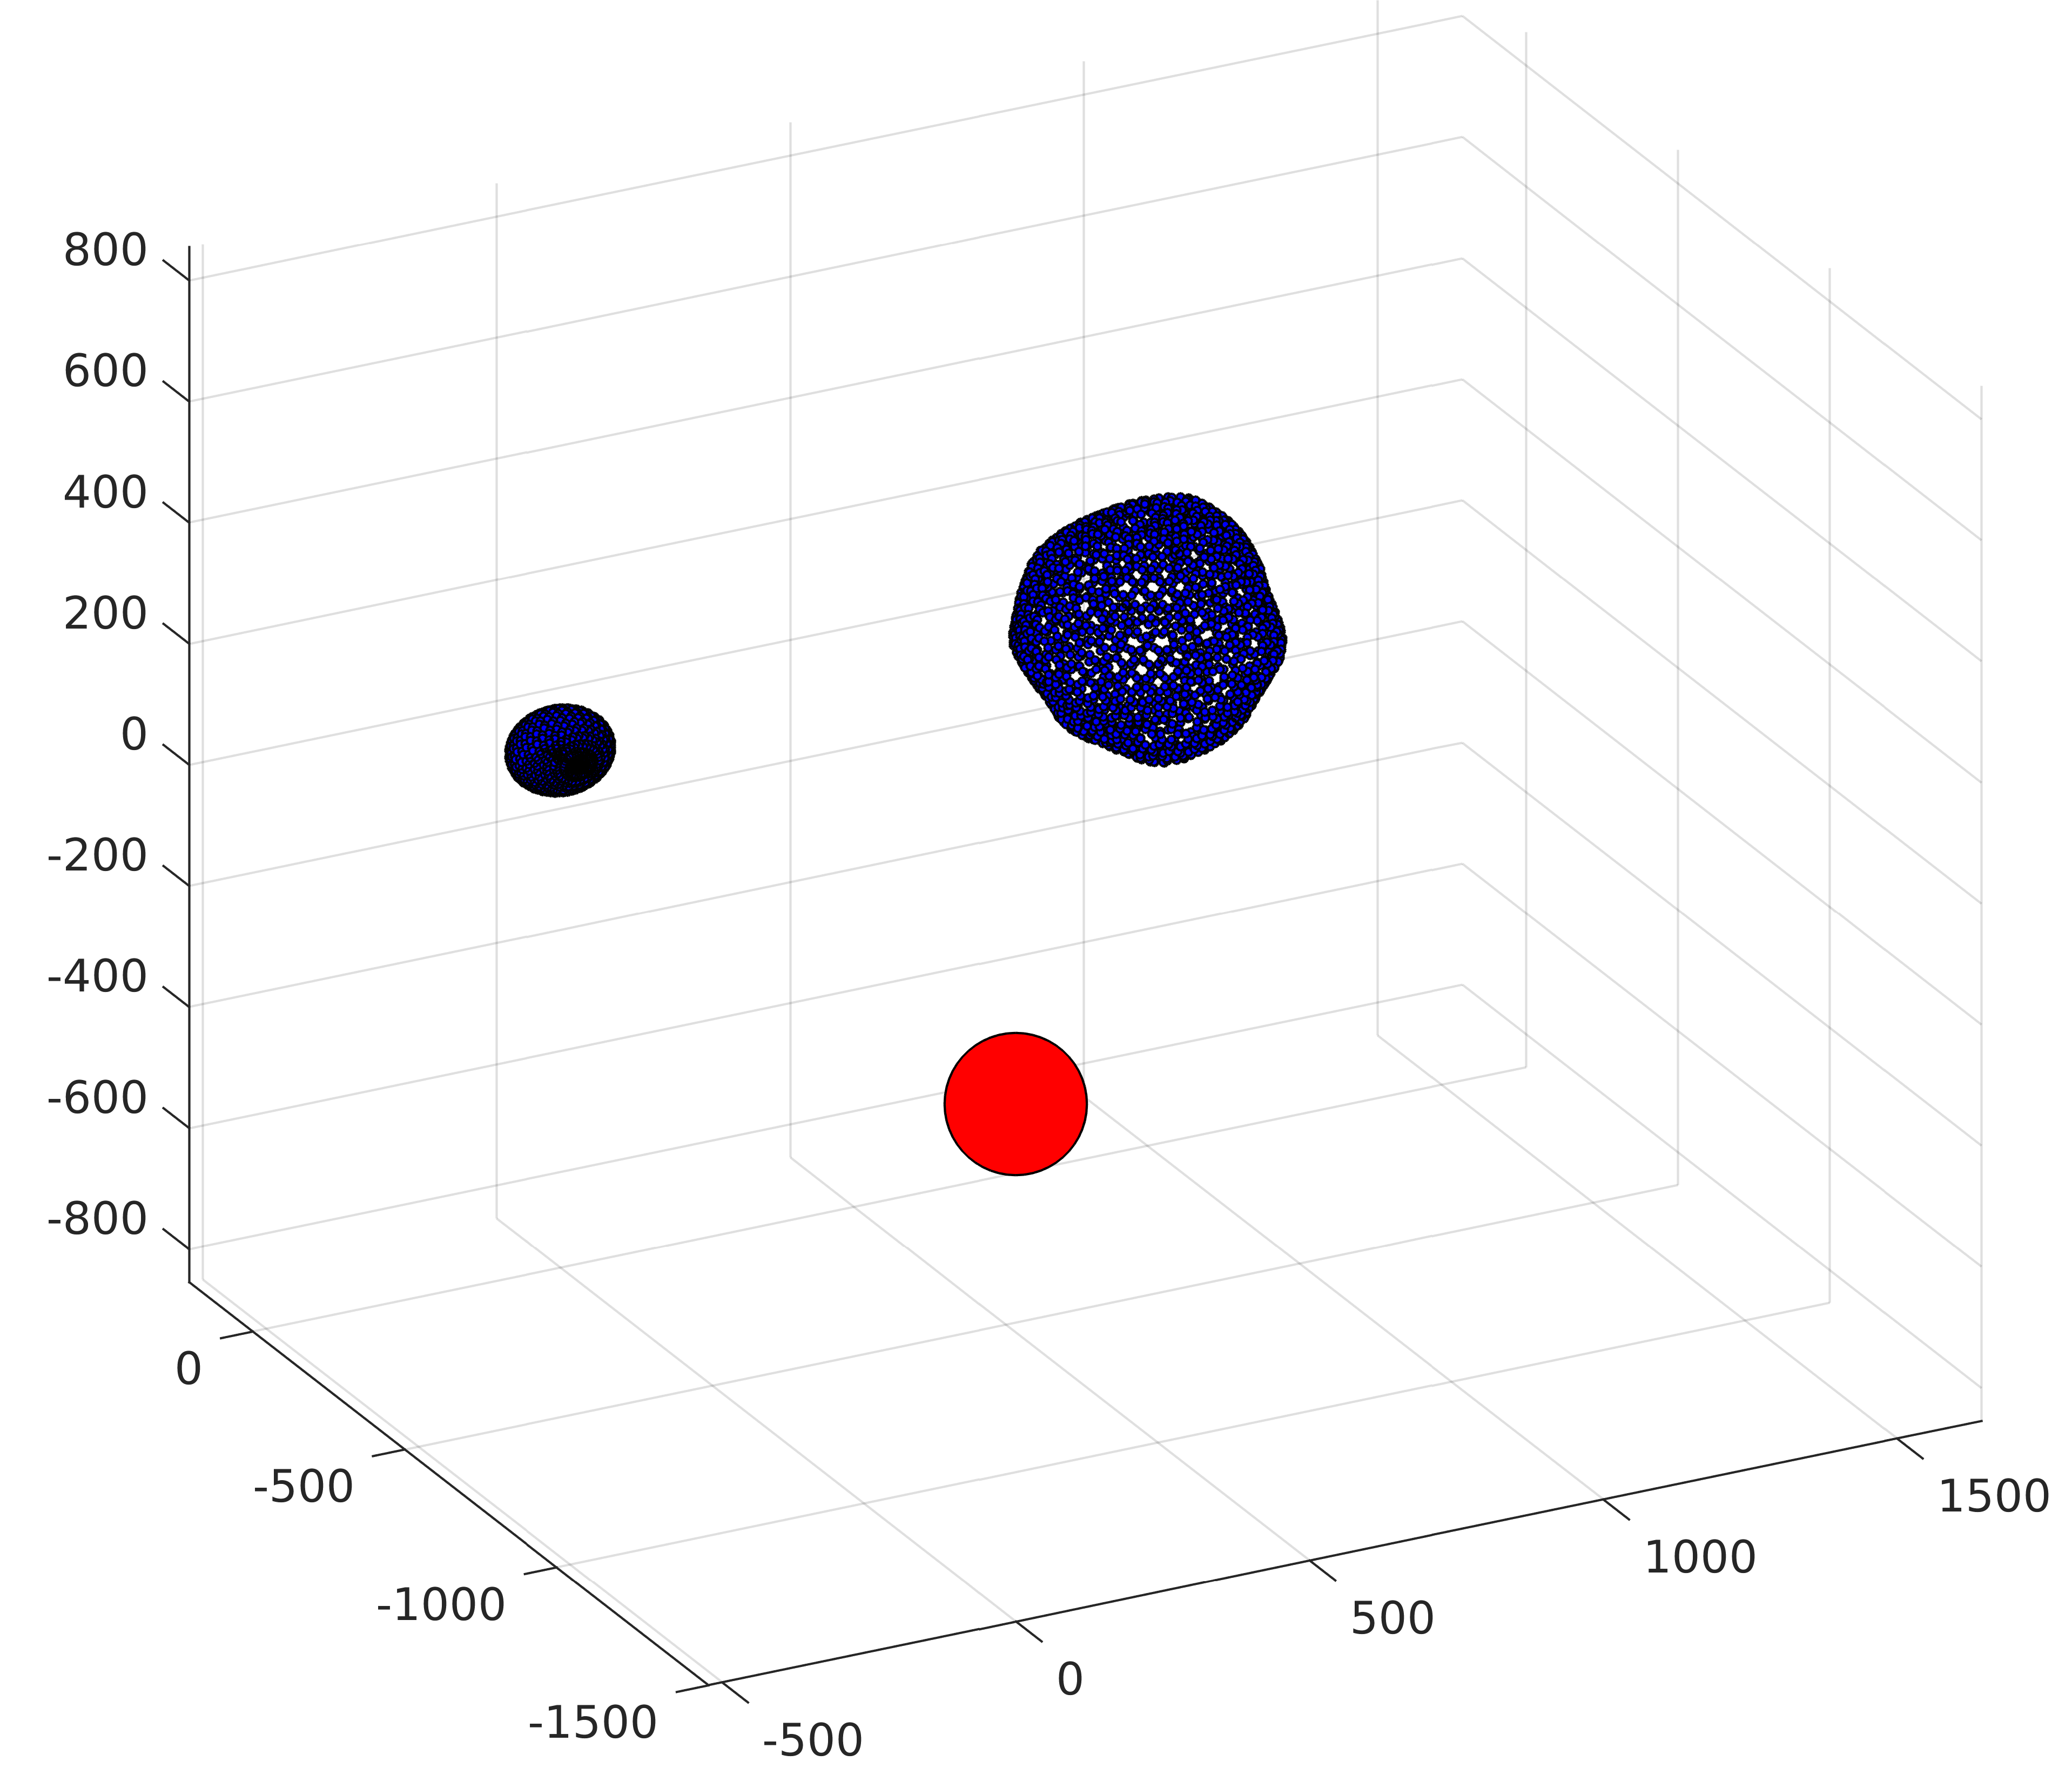
\includegraphics[width=\linewidth]{rsc/mutual_model.png}
    \captionof{figure}{The binary system of asteroids Didymos with the Sun direction. Latest shape models of the ESA have been used in this simulation. The primary has a radius of 500 meters and the secondary 80 meters.}
    \label{fig:4.2}
\end{center}
After implementation of the revolution of Didymoon, the following results are obtained for the surface temperatures of the secondary including the mutual heating from the primary:
\begin{center}
    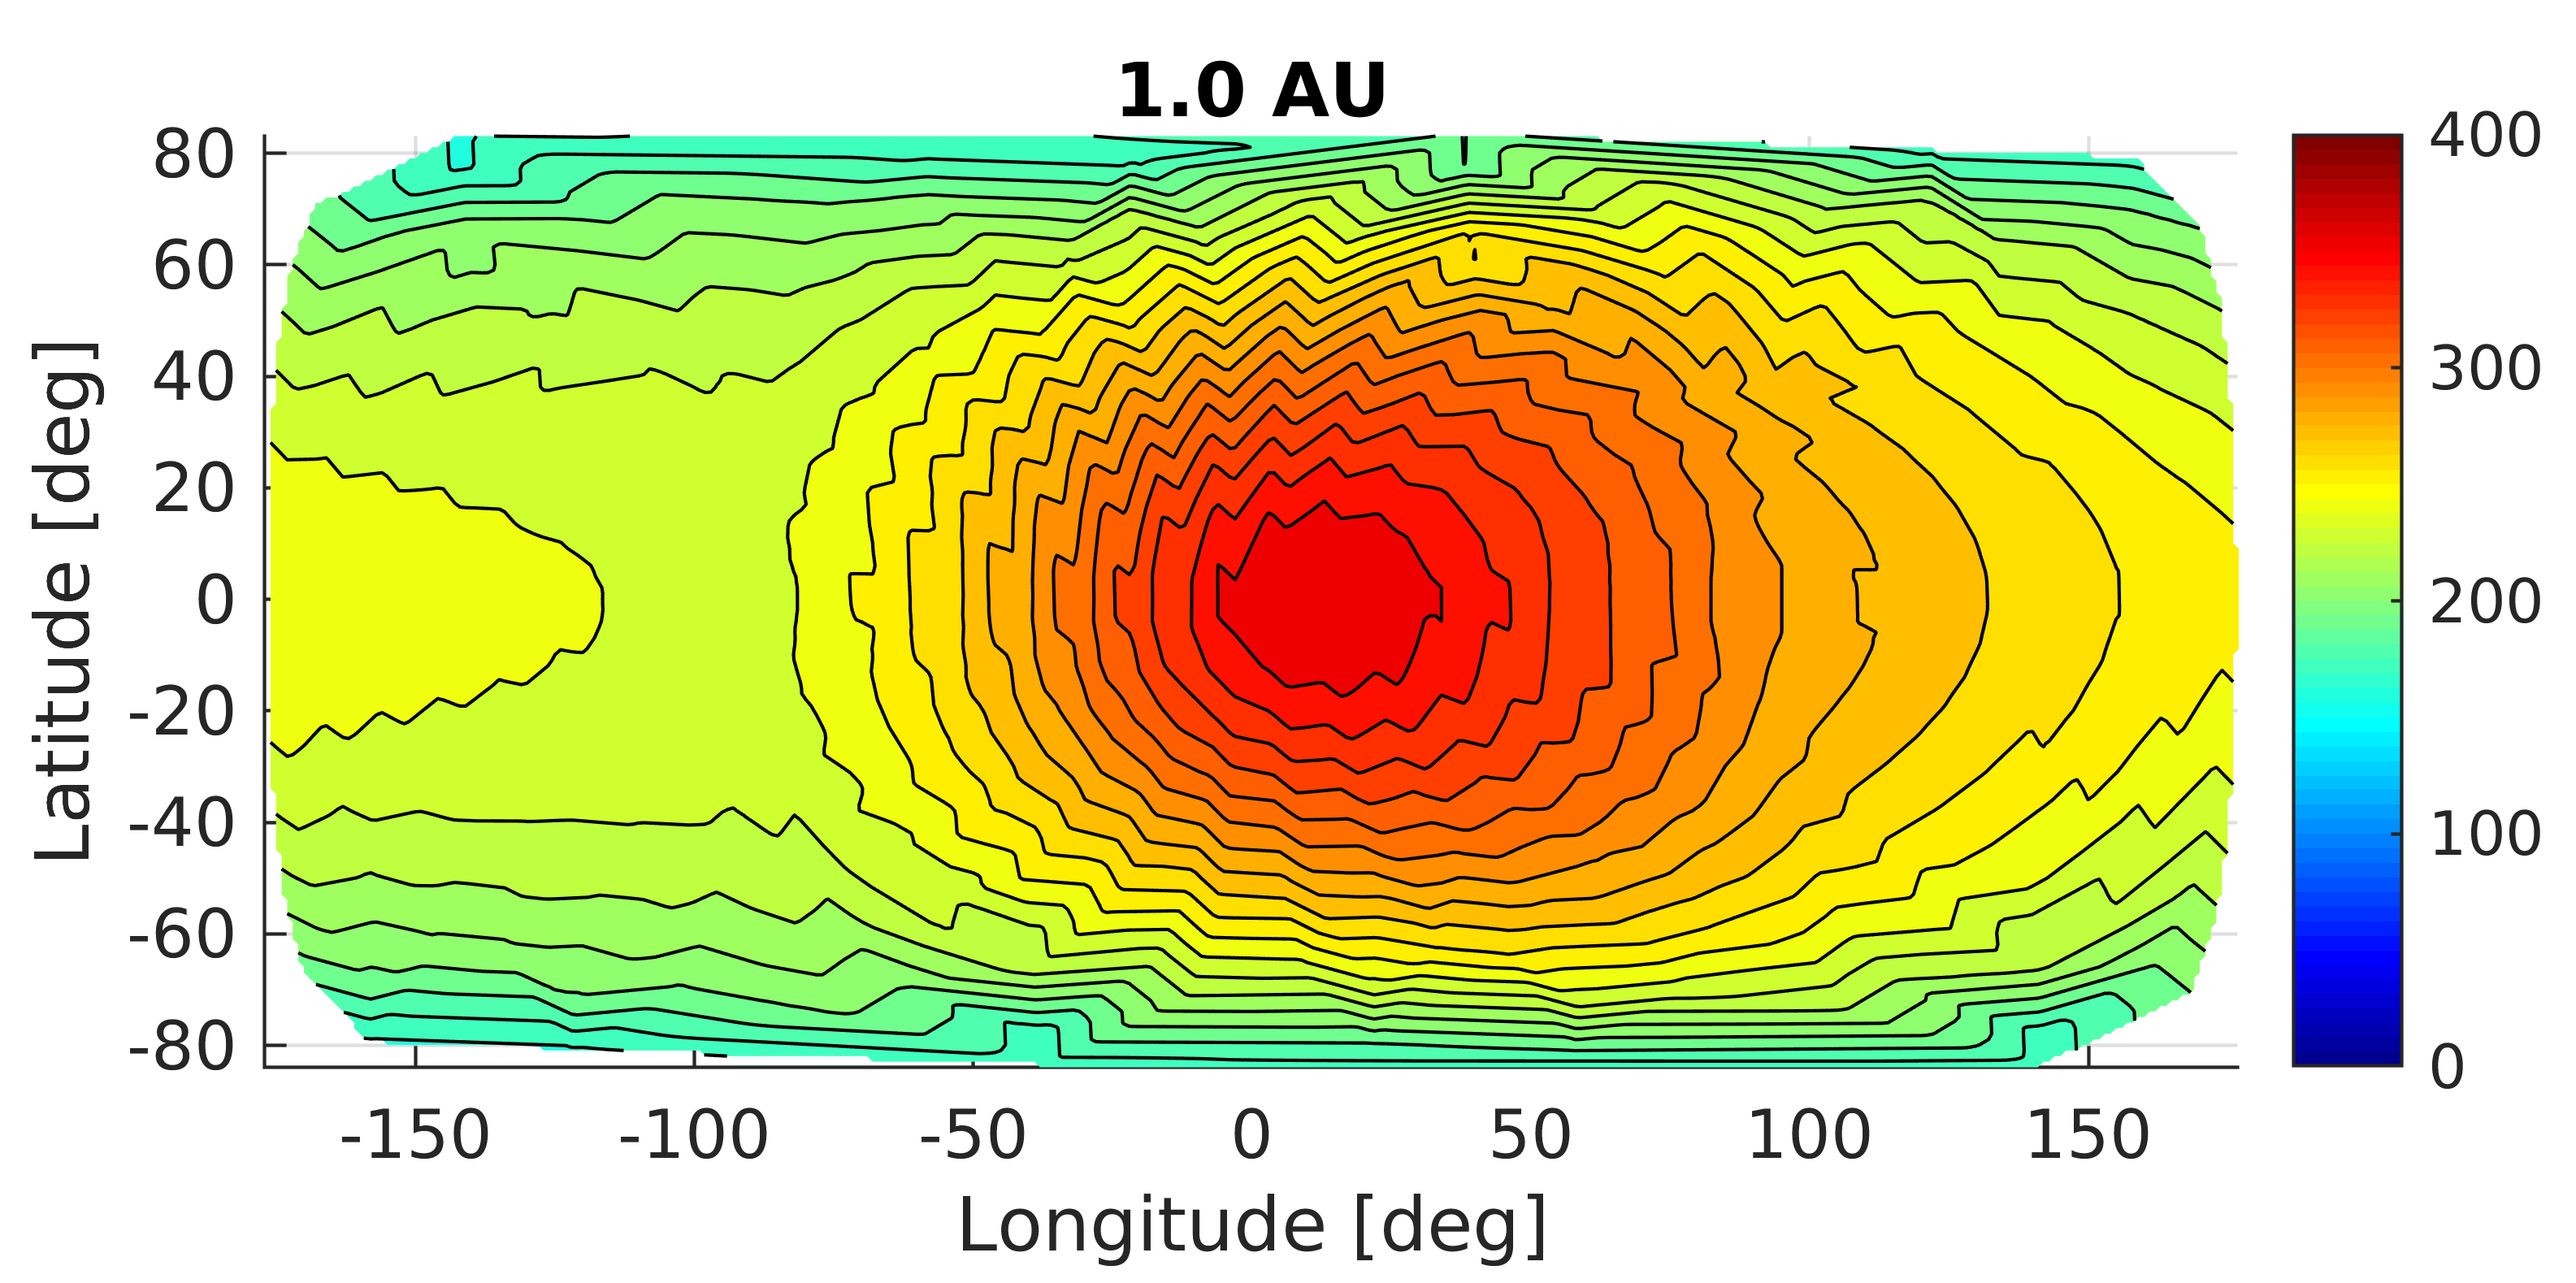
\includegraphics[width=\linewidth]{rsc/mutual.png}
    \captionof{figure}{Thermal map of the secondary of the binary system of asteroids Didymos including the mutual heating from the primary using ESA shape models.}
    \label{fig:4.2}
\end{center}
The computation were realized without the implementation of the obliquity, which is discussed in next parts. To compare with the previous implementation in \autoref{eq:2.1}, this graphs shows the benefits of including the mutual heating:
\begin{center}
    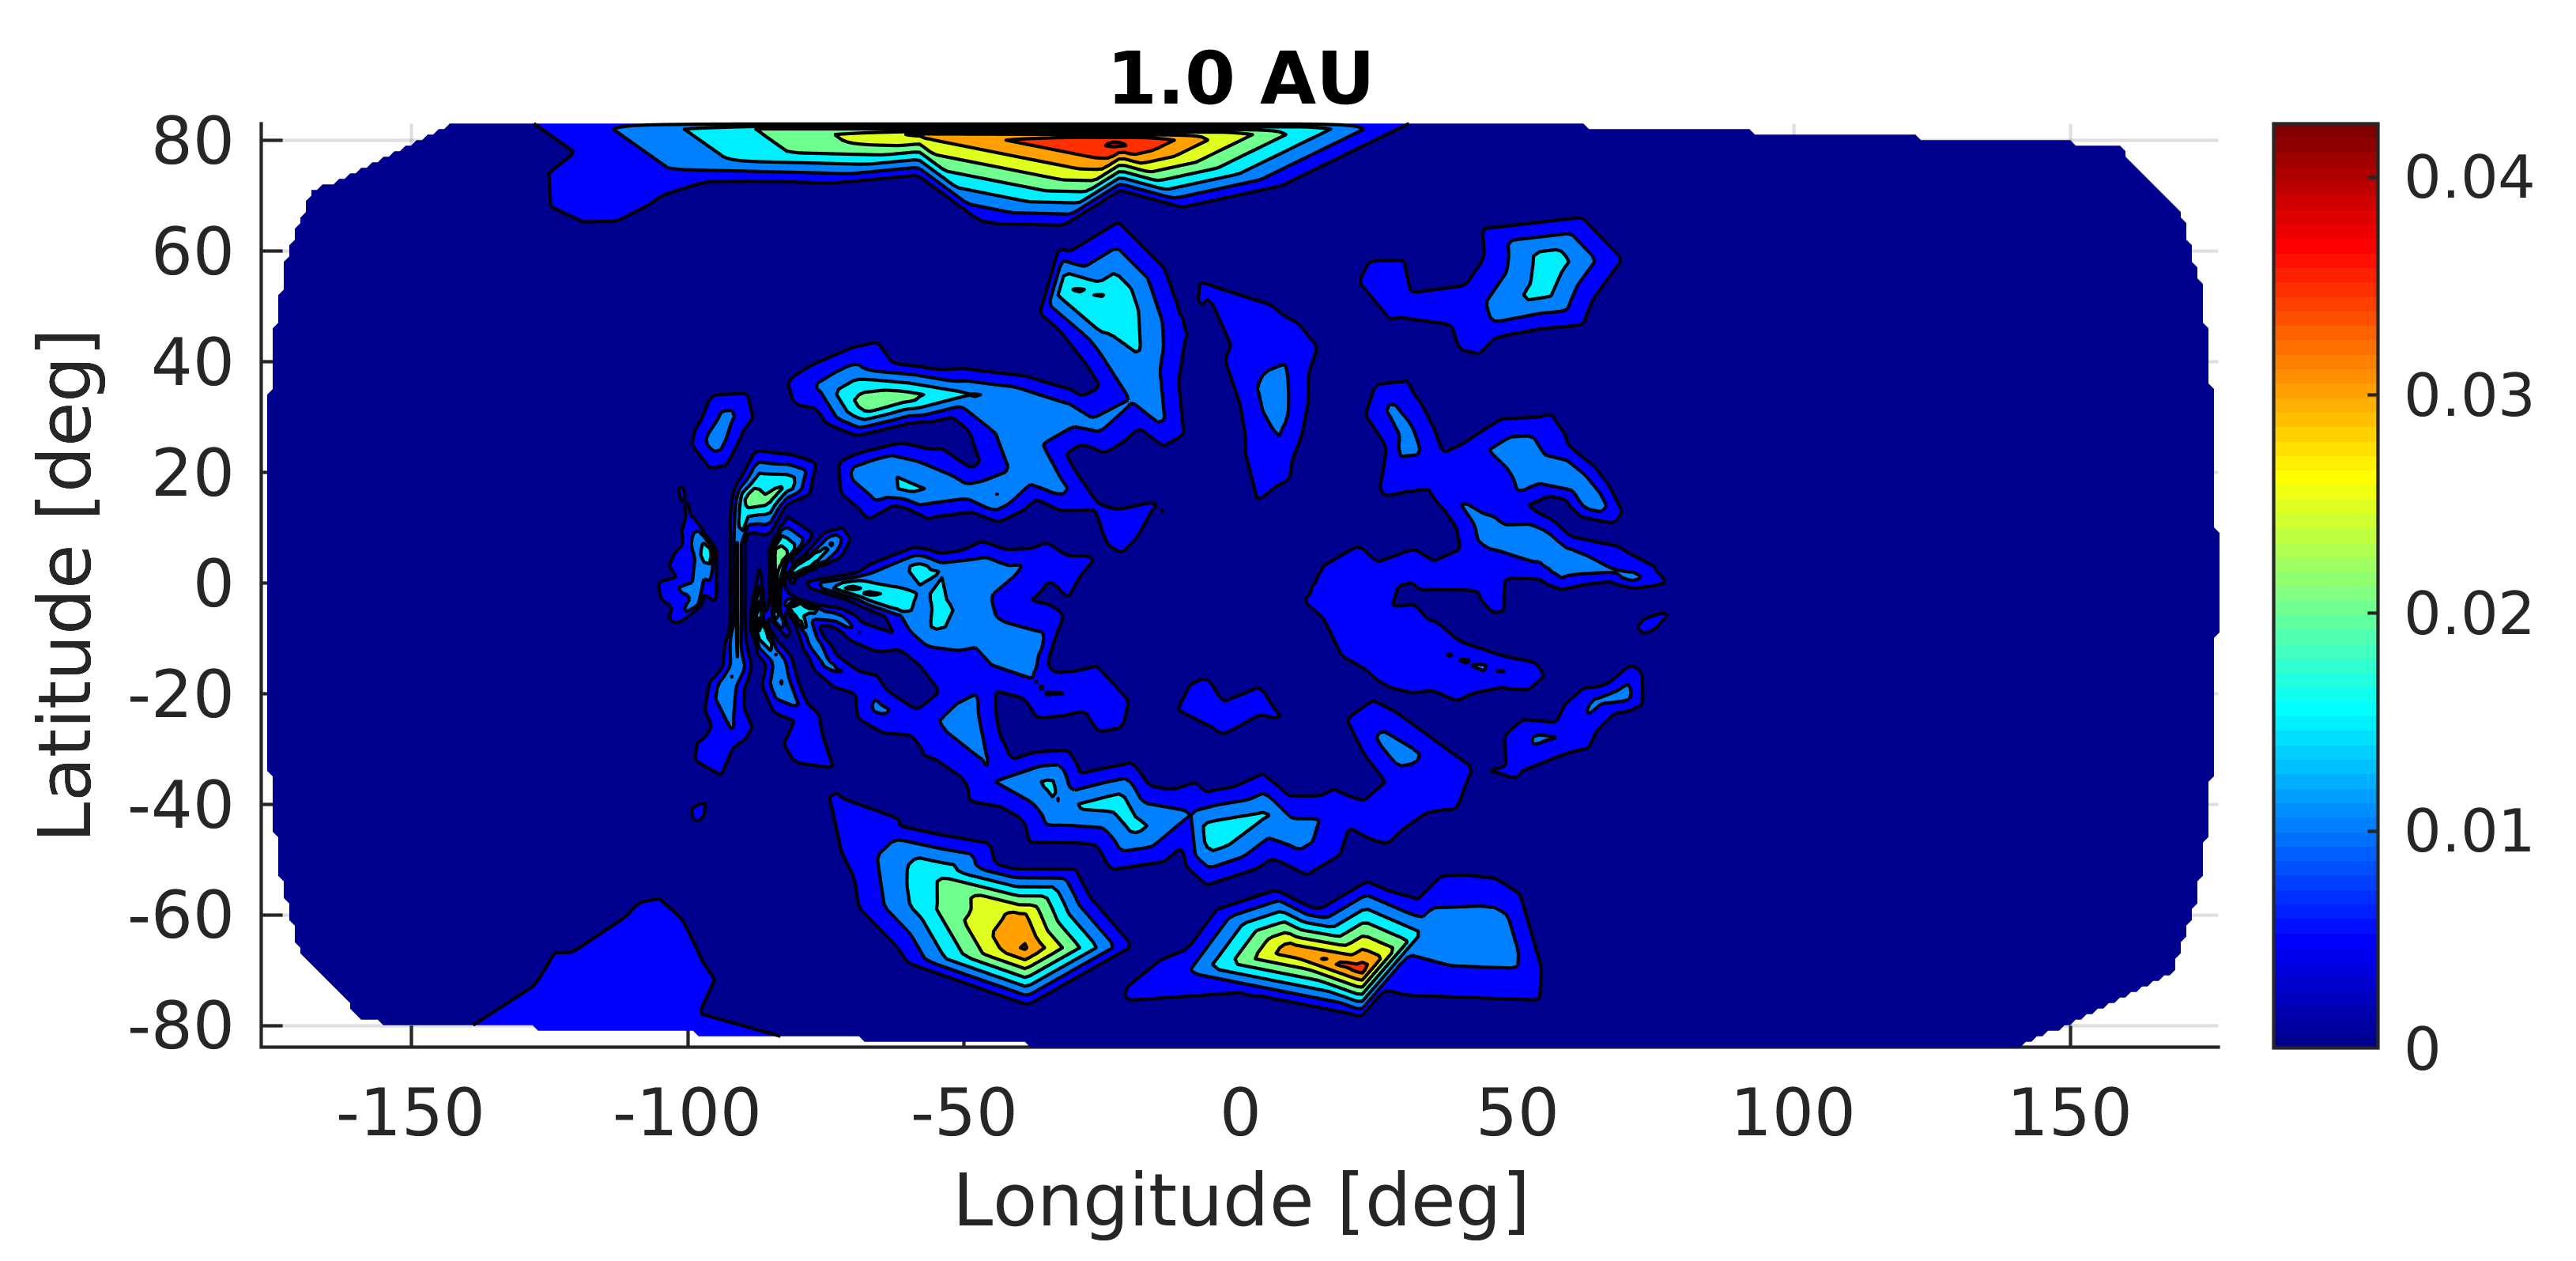
\includegraphics[width=\linewidth]{rsc/mutual_W.png}
    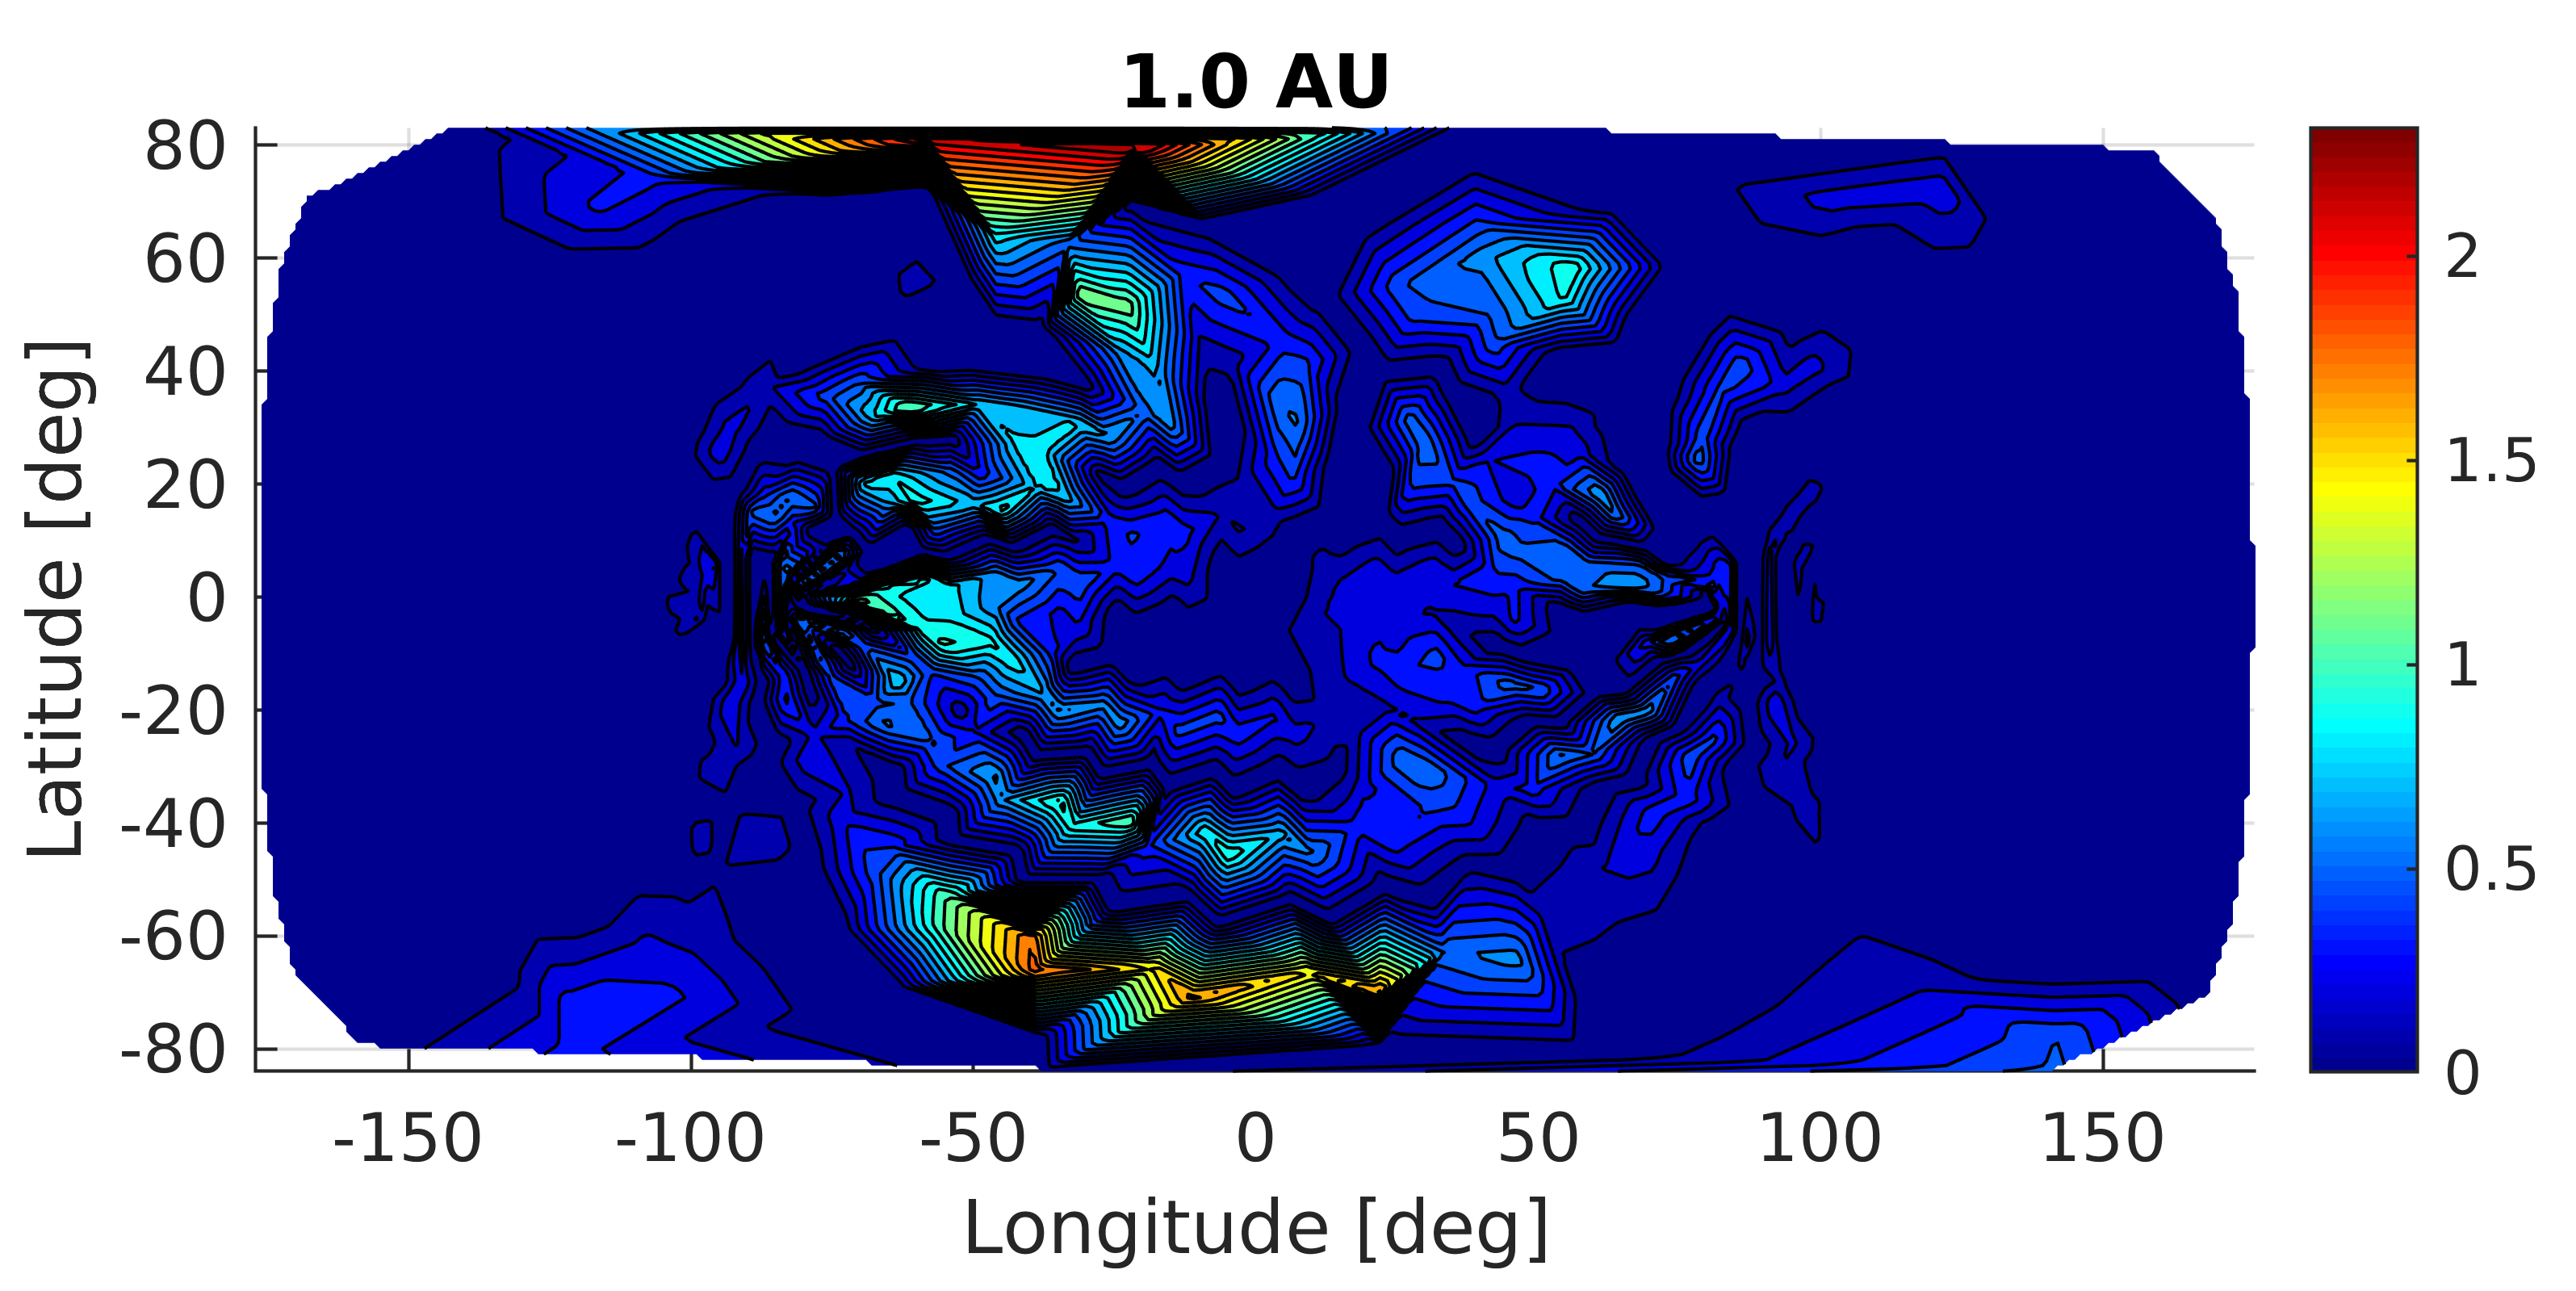
\includegraphics[width=\linewidth]{rsc/mutual_Wu.png}
    \captionof{figure}{The two graphs shows the impact of including the mutual heating on the surface temperatures of Didymoon. The first figure shows the difference between the surface temperatures with the secondary diffuse mutual heating only (\autoref{eq:4.2}) and without it. The second image is the difference of temperature including the two equation of the mutual heating (\autoref{eq:4.2} \& \autoref{eq:4.4}) and without it.} 
    \label{fig:4.2}
\end{center}
The assumptions which consisted of considering the direct mutual heating as the largest flux of the mutual is confirmed with this graph. Furthermore, the \autoref{eq:4.2} costs much more computational time rather than the \autoref{eq:4.4}, thus, and due to the present albedo, it might be more clever to not implement it. The first case suggests an increase of $0.05$ \si{\kelvin} where the second case represents an increase of more than $2$ \si{\kelvin} depending on the regions.
